\chapter{Results and Discussion}

\section{Introduction} 

This chapter presents obtained results. Through the experiments with eligible volunteers, a set of important quantitative metrics were collected, which allows an evaluation, based on PMRT. Qualitative data were obtained from the survey filled by the volunteers and therapist about the system acceptance and limitations during their trial experience.

\section{Trials performance evaluation information}

Table \ref{tb:ResultsPMRT} present the performance evaluation realized by the therapist.

\begin{table}[!htbt]
\caption{PMRT Evaluation Summary} \label{tb:ResultsPMRT}
\centering
\begin{tabular}{cccccc}
\toprule
Participant & Protocol / Tasks & Command & Collision & Time(s) & Score(\%) \\ \midrule
\multirow{4}{*}{1} & 1.1   & 38 & 2 & 199 & 50 \\
                            			     & 2.1 & 37 & 1 & 328 & \multirow{2}{*}{50}\\
                            			     & 2.2 &  7 & 0 & 57  & \\
						     & 3.1   & 54 & 0 & 354 & 75 \\ \midrule
\multirow{4}{*}{2} & 1.1   & 27 & 0 & 282 & 75 \\
                            			     & 2.1 & 17 & 0 & 127 & \multirow{2}{*}{75}\\
                            			     & 2.2 & 21 & 0 & 67  & \\
						     & 3.1   & 66 & 0 & 178 & 75 \\ \midrule
\multirow{4}{*}{3} & 1.1   & 14 & 0 & 227 & 75 \\
                            			     & 2.1 & 9  & 0 & 98 & \multirow{2}{*}{50}\\
                            			     & 2.2 & 13 & 0 & 51  & \\
						     & 3.1   & 34 & 0 & 236 & 75 \\ 
\bottomrule
\end{tabular}
\end{table}


\section{System requirements information}
Figures \ref{fig:sGooExcel} and  \ref{fig:sLimExcel} represent  the average and standard deviation value of each participants’ evaluation based on survey questionnaire questions present by Tables \ref{table:tbSurvey01} and \ref{table:tbSurvey02} in Section \ref{sec:procedureProcess}.  Figures  \ref{fig:sGooWC} and \ref{fig:sLimWC} represents visual qualitative information about advantages, disadvantages and comments inputed of each training experiment performed by the user's. The questions applied were divided into two groups: good aspects or limiting aspects. Where, for questions where the average value was greater than or equal to three, it is considered good; otherwise, it was considered a limitation.

\begin{figure}[!htbp]
\center
\begin{minipage}{0.495\linewidth}
\center
\captionsetup{justification=centering,margin=0.5cm,font=small}
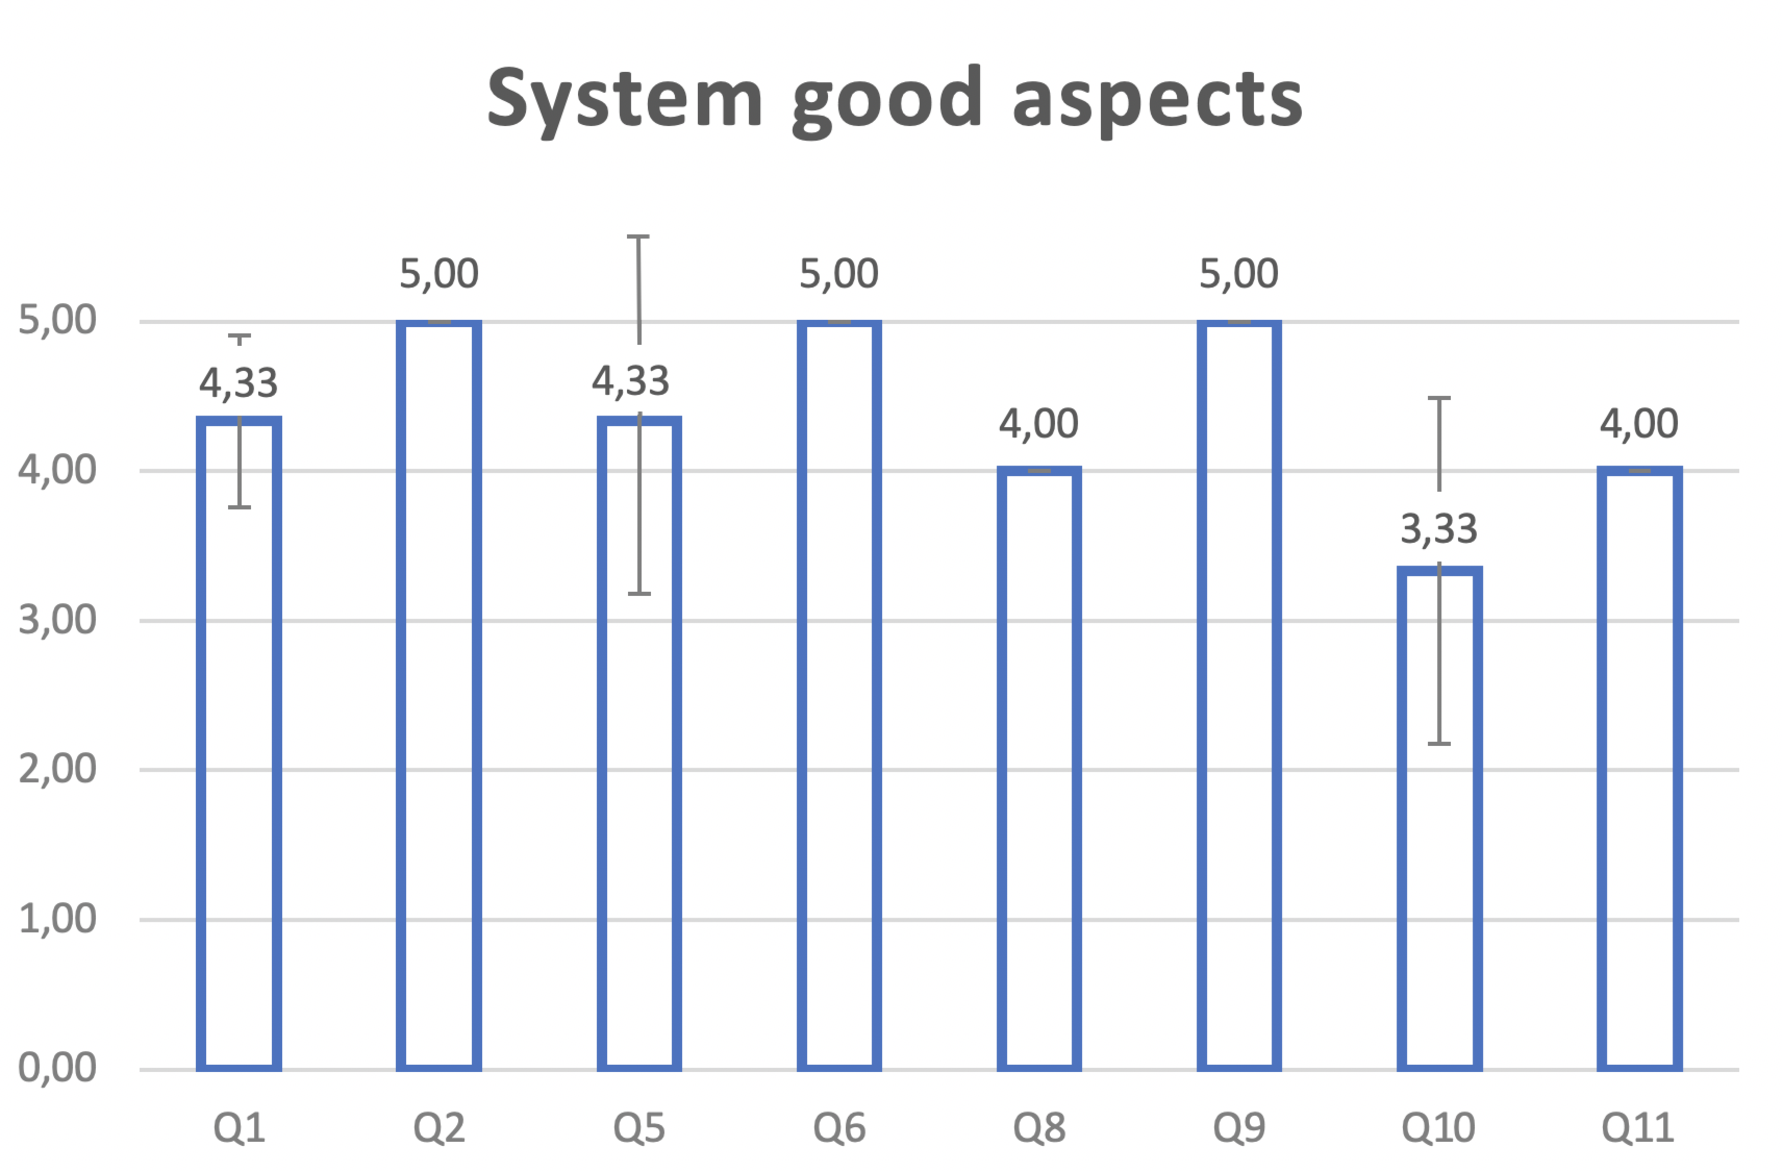
\includegraphics[width=1\linewidth]{img/cap6/sGoodAspExcel}
\caption{System Good Aspects} \label{fig:sGooExcel}
\end{minipage}
\begin{minipage}{0.495\linewidth}
\center
\captionsetup{justification=centering,margin=0cm,font=small}
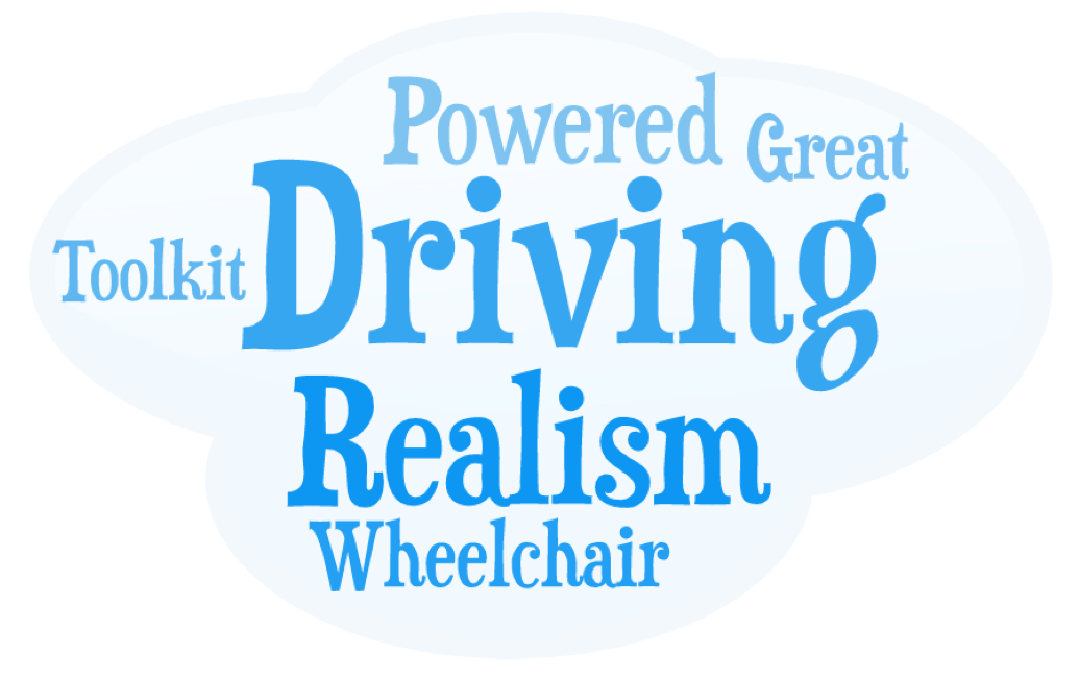
\includegraphics[width=1\linewidth]{img/cap6/sGoodAspWordClouds}
\caption{Good evaluations} \label{fig:sGooWC}
\end{minipage}
\end{figure}


\begin{figure}[!htbp]
\center
\begin{minipage}{0.495\linewidth}
\center
\captionsetup{justification=centering,margin=0.5cm,font=small}
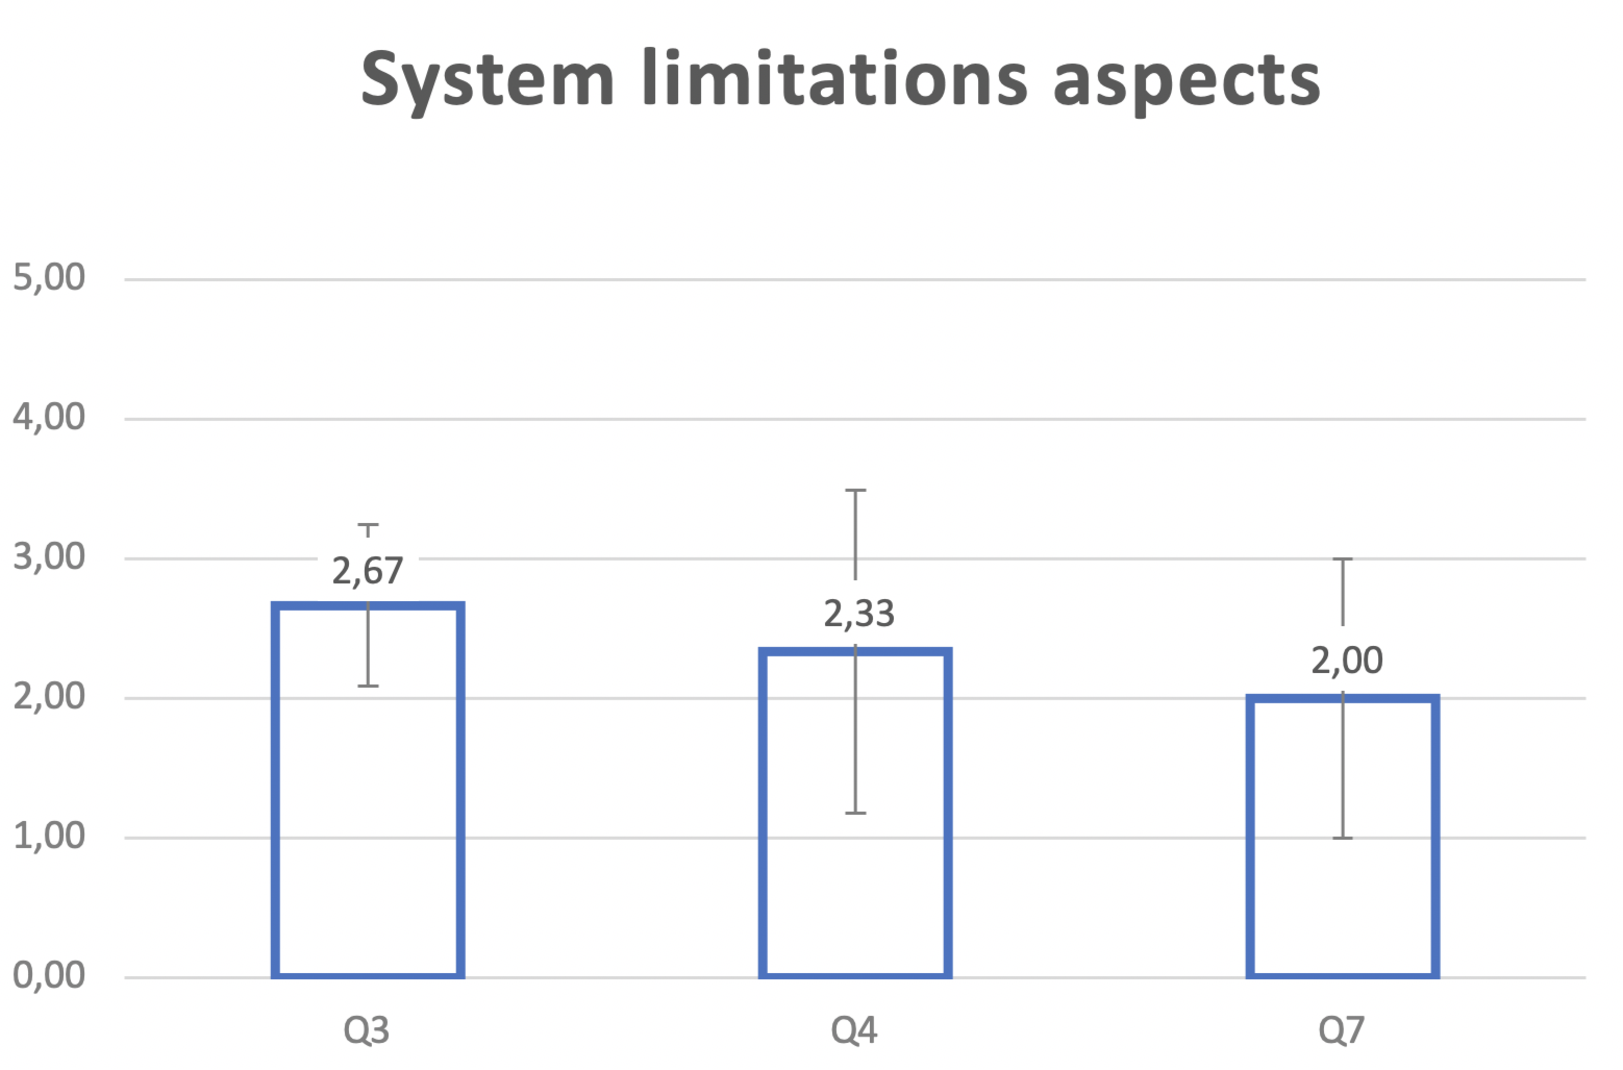
\includegraphics[width=1\linewidth]{img/cap6/sLimitationAspExcel}
\caption{System Limitations Aspects} \label{fig:sLimExcel}
\end{minipage}
\begin{minipage}{0.495\linewidth}
\center
\captionsetup{justification=centering,margin=0cm,font=small}
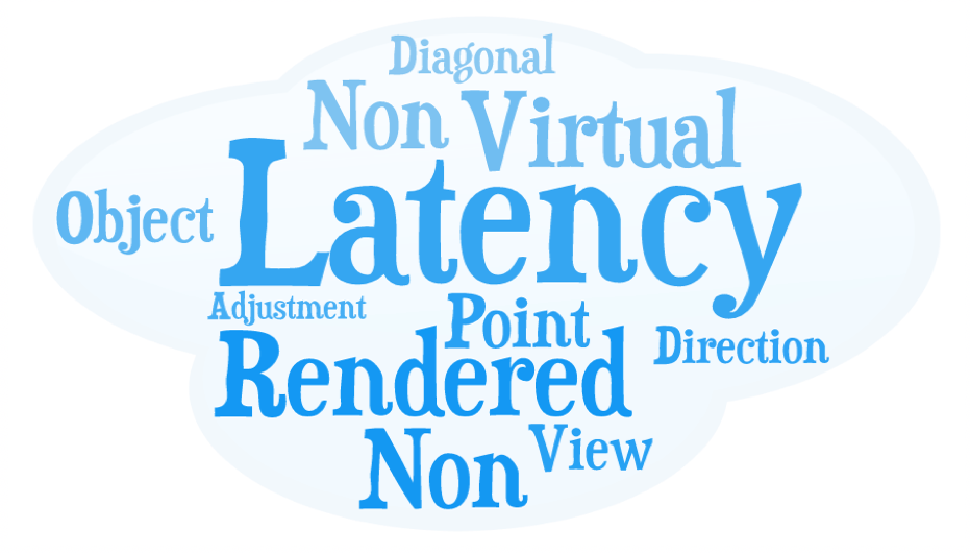
\includegraphics[width=1\linewidth]{img/cap6/sLimitationAspWordClouds}
\caption{System limitations evaluations} \label{fig:sLimWC}
\end{minipage}
\end{figure}


The discussion around the extracted graphic data that represents the users' evaluation will be carried out in Section \ref{sec:discussion}.

\section{{Protocols evaluation}}

\subsection{{Electrodermal Activity  Analysis}}

The ISCR (obtained after processing EDA) Descriptive Statistics is presented in Table \ref{table:tbISCR} \cite{braithwaite2015}. It is possible to observe that Skin Conductance Responses are skewed and can produce non-normal distributions \cite{braithwaite2015}, as observed in the difference between ISCR average and ISCR median.


\begin{table}[!htb]
\caption {ISCR Descriptive Statistics}\label{table:tbISCR}
\centering
\begin{tabular}{ccccc}
\toprule
Group & Count & Mean &SD & Median \\
\midrule
Protocol 01 &  83 & -4.65e-18 & 0.988 & -0.110 \\
Protocol 02 & 111 & -9.01e-12 & 0.991 & -0.263 \\
Protocol 03 & 123 & -2.44e-11 & 0.992 & -0.274 \\
\bottomrule
\end{tabular}
\end{table}

Columns meaning:

\begin{itemize}
\item Count: number of observations;
\item Mean: ISCR average on each protocol;
\item SD: Standard Deviation of ISCR on each protocol; and
\item Median: ISCR Median of each protocol.
\end{itemize}

Results of statistical analysis of ISCR as a variable in each protocol are: \textbf{Kruskal-Wallis chi-squared = 0.012995, df = 2, p-value = 0.9935}, showing no statistical significant differences between each protocol applied related to ISCR \cite{bodkin2019}.
These results refer only to the sample utilized, to demonstrate system's capabilities. A higher number of volunteers in future studies will be necessary to draw broader and more general conclusions. Therefore, future studies should consider a higher number of participants.
\newline


\subsection{Stress Index Analysis}

It is important to monitor subject conditions during training to be able to safely conduct activities and to objectively determine causes of failure during wheelchair driving in order to provide a course of action towards acquisition of good driving skills \cite{affanni2018,healey2005}. 

Stress (both physical and psychological) affects subject abilities to safely drive vehicles, and driving PW is no different. Some studies were conducted aiming to provide stress measures using biosignal monitoring and processing \cite{healey2005}. 

It is not an objective of this work to propose a new stress measure. Instead, was used a stress measure already discussed in the literature \cite{baevsky2008} that is easily obtainable through a free version software Kubios \cite{kubios2017}.

Aiming obtain the stress index for each protocol and each participant, we used the IBI time series prepared for processing using Kubios.

Table \ref{table:stZones} present the Stress Zone and corresponding SI (Stress Index) band values.


\begin{table}[!htb]
\caption{Stress zone boundaries  \cite{hrvKubios2018}} \label{table:stZones}
\centering
\begin{tabular}{cc}
\toprule
Stress Zones   & SI     \\
\midrule
Very High &  >30         \\
High      &  22.4 - 30   \\
Elevated  &  12.2 - 22.4 \\
Normal    &  7.1 - 12.2  \\
Low       &  <7.1        \\
\bottomrule
\end{tabular}
\end{table}

Participants comparison results are presented in Table \ref{table:uSResults}:

\begin{table}[!htb]
\caption{Stress zone participants comparison}\label{table:uSResults}
\centering
\begin{tabular}{cccc}
\toprule
User & SI & SI & SI\\
& Protocol 1 & Protocol 2 & Protocol 3\\
\midrule
Participant  1 & 12.0769 & 11.4139 & 9.9194 \\
Participant  2 & 17.5959 & 14.8135 & 16.9240 \\
Participant  3 & 6.0430 & 5.2265  & 8.0705 \\
\bottomrule
\end{tabular}
\end{table}

Finally, data presented on Table \ref{table:uSResults} is translated to stress zones in Table \ref{table:trcSZ}:

\begin{table}[!htb]
\caption{Stress zone participants translation}\label{table:trcSZ}
\centering
\begin{tabular}{cccc}
\toprule
User & SI & SI & SI\\
& Protocol 1 & Protocol 2 & Protocol 3\\
\midrule
Participant  1 & Normal & Normal & Normal \\
Participant  2 & Elevated & Elevated & Elevated \\
Participant  3 & Low & Low & Normal \\
\bottomrule
\end{tabular}
\end{table}

All participants did not have a significant change in their stress index between protocols, which supports the conclusion that the protocols might not have an impact on subject’s stress. A bigger sample can support more strongly this conclusion, which can be done in future studies.

\section{Discussion}
\label{sec:discussion}

To better understand the participant's acceptance of the developed tool/architecture and its requirements, the following considerations are presented.

Questions 1, 2  (Figure \ref{fig:sGooExcel}) and 3  (Figure \ref{fig:sLimExcel})  seek to evaluate usability. It is possible to note that the participants considered the GUI handy and that the system is easy to learn. According to participants, the two main faults in the system were the latency (response time - Q7 (Figure \ref{fig:sLimExcel})) and failure to render virtual objects  (Figure \ref{fig:sLimWC}) shown in Figures \ref{fig:errorRender01}, \ref{fig:errorRender02} and \ref{fig:errorRender03}.  
In Figure \ref{fig:errorRender01}, the guidance arrow is rendered at a wrong place, in Figure \ref{fig:errorRender02} and \ref{fig:errorRender03} the guidance and final activity arrows were not rendered properly, due to image quality, marker size or illumination. Other facts can be considered, with less relevance such as the PW does not possess diagonal movements Q4  (Figure \ref{fig:sLimExcel})  and adjustments from the participant  (Figure \ref{fig:sLimWC}).

On the other hand, questions 5, 6, 8, 10 and 11  (Figure \ref{fig:sGooExcel})  confirm that the application of telerehabilitation techniques fused with the AR techniques present  itself as a great tool to support the users driving skills improvement, without leaving their home, in agreement with participants evaluations in Figures \ref{fig:sGooExcel} and \ref{fig:sGooWC}. 

\begin{figure}[!htbp]
\center
\begin{minipage}{0.495\linewidth}
\center
\captionsetup{justification=centering,margin=0.5cm,font=small}
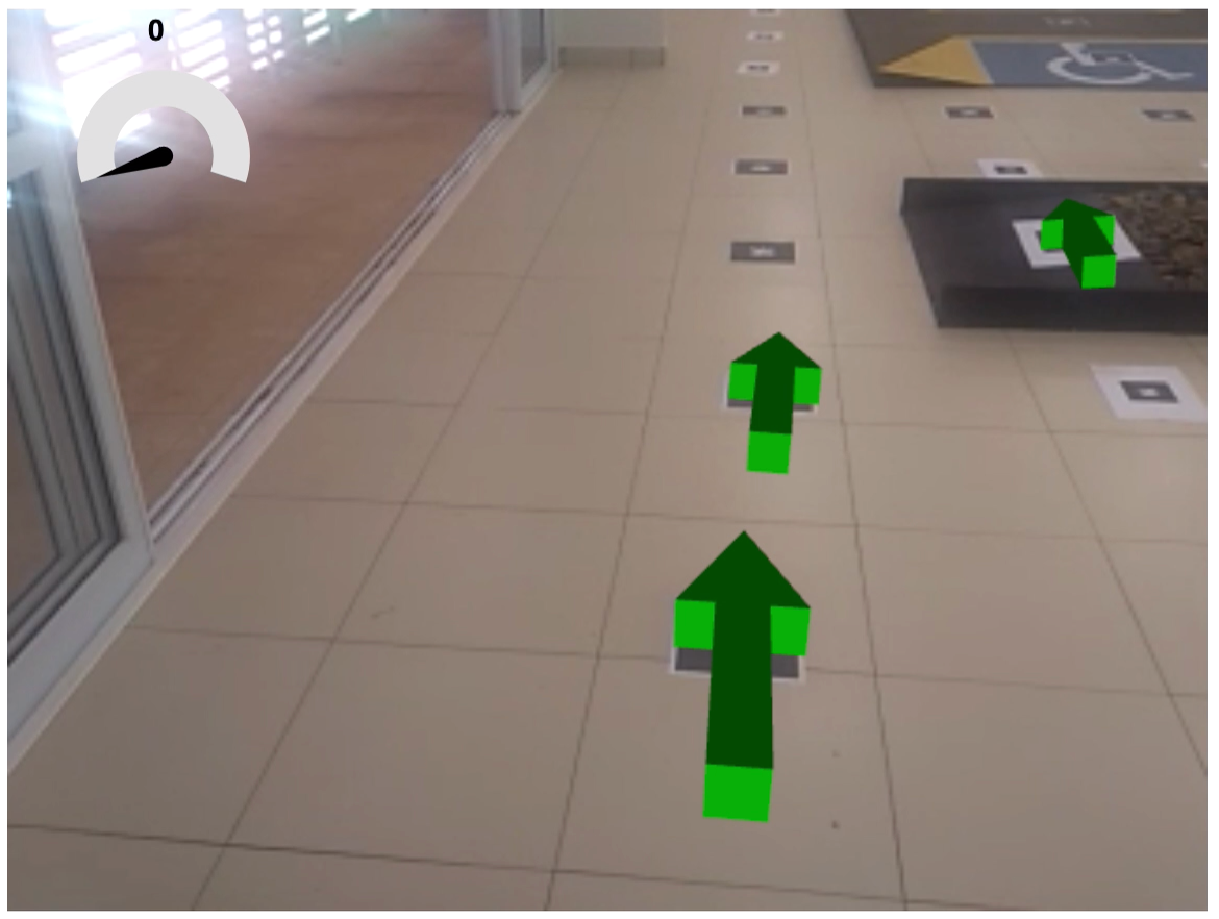
\includegraphics[width=1\linewidth]{img/cap6/errorRender01}
\caption{Rendering failure-01} \label{fig:errorRender01}
\end{minipage}
\begin{minipage}{0.495\linewidth}
\center
\captionsetup{justification=centering,margin=0cm,font=small}
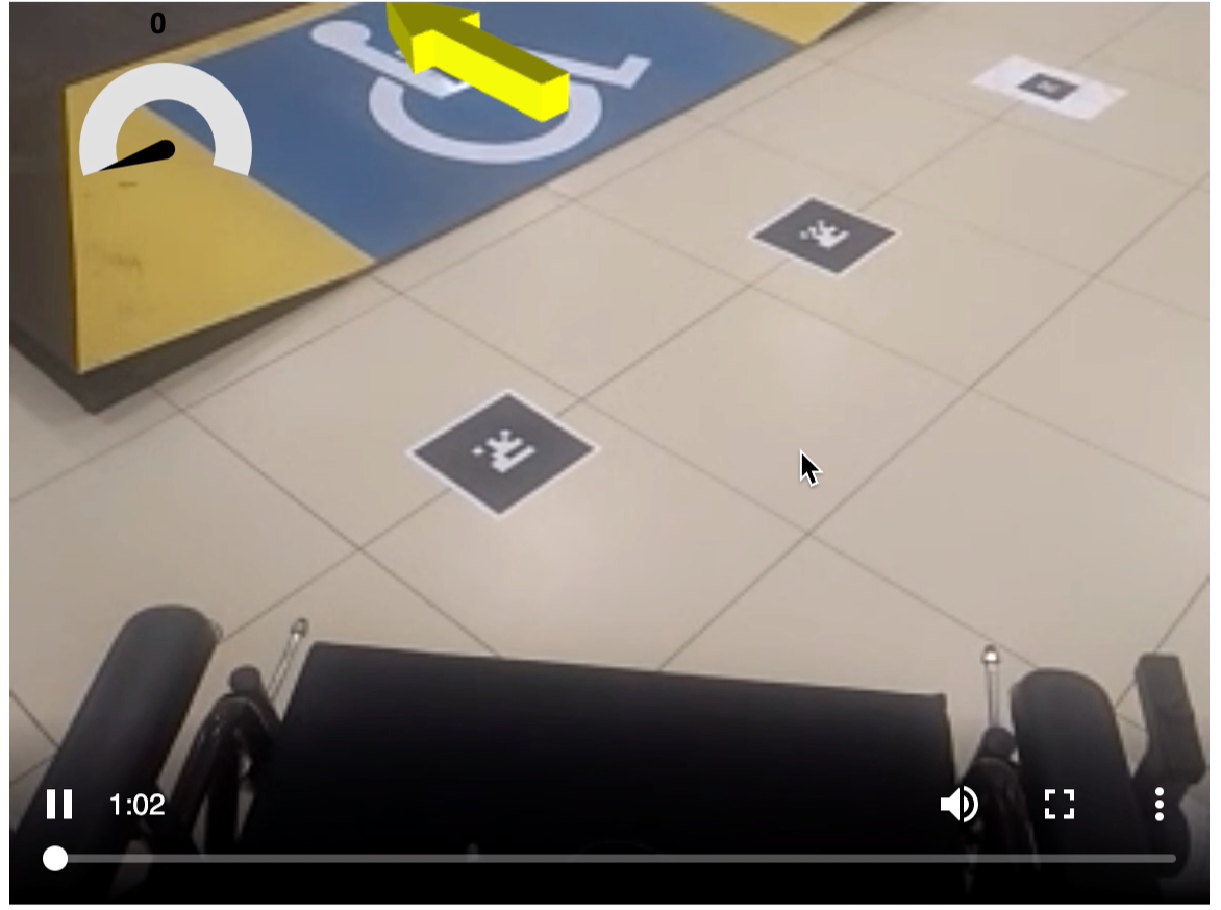
\includegraphics[width=1\linewidth]{img/cap6/errorRender02}
\caption{Rendering failure-02} \label{fig:errorRender02}
\end{minipage}
\begin{minipage}{0.495\linewidth}
\center
\captionsetup{justification=centering,margin=0cm,font=small}
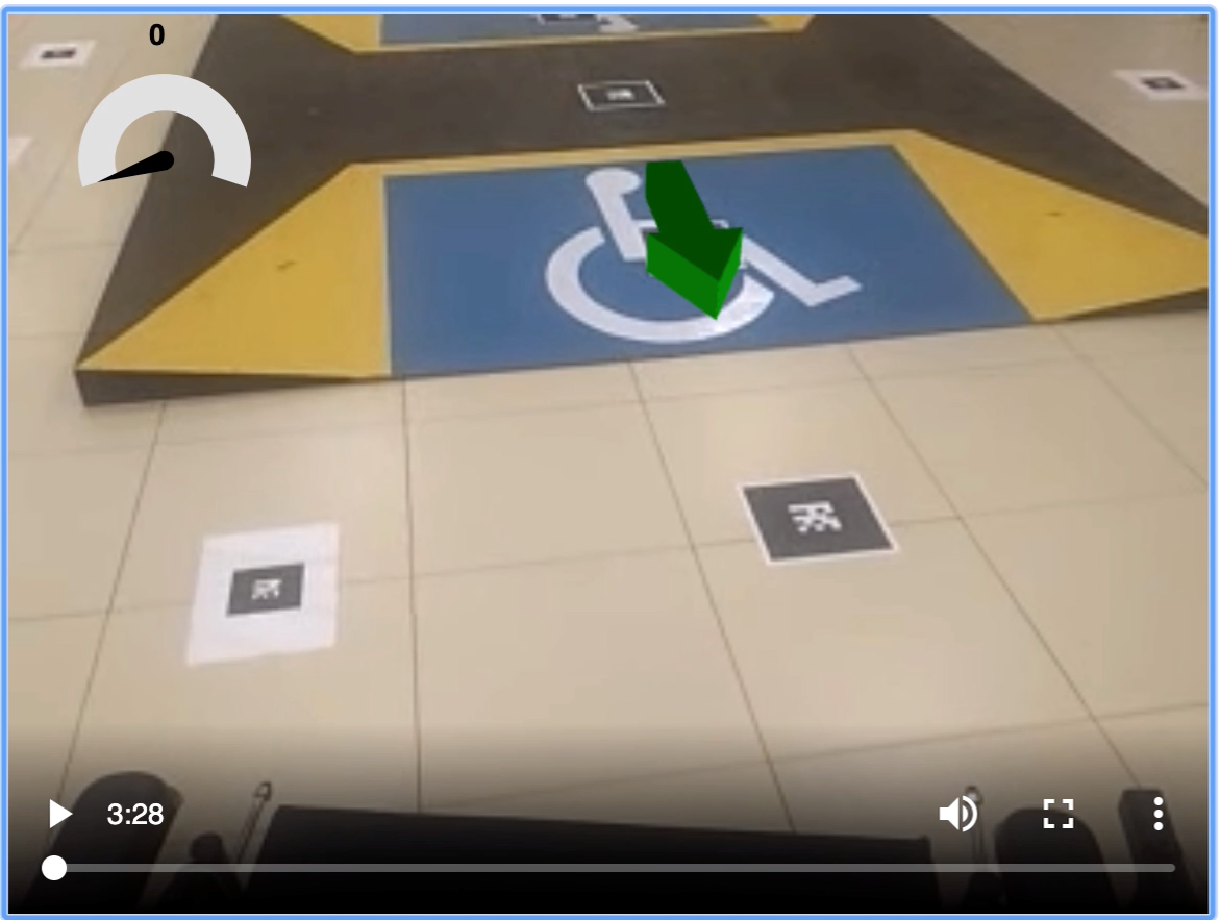
\includegraphics[width=1\linewidth]{img/cap6/errorRender03}
\caption{Rendering failure-03} \label{fig:errorRender03}
\end{minipage}
\end{figure}

This is due to the realism, by controlling a real PW, through a real scenario, in addition to listening to the sounds of triggering and pausing the PW, during the training execution, as shown in Figures \ref{fig:endFirstAct} and \ref{fig:spingWAct}.

\begin{figure}[!htbp]
\center
\begin{minipage}{0.495\linewidth}
\center
\captionsetup{justification=centering,margin=0.5cm,font=small}
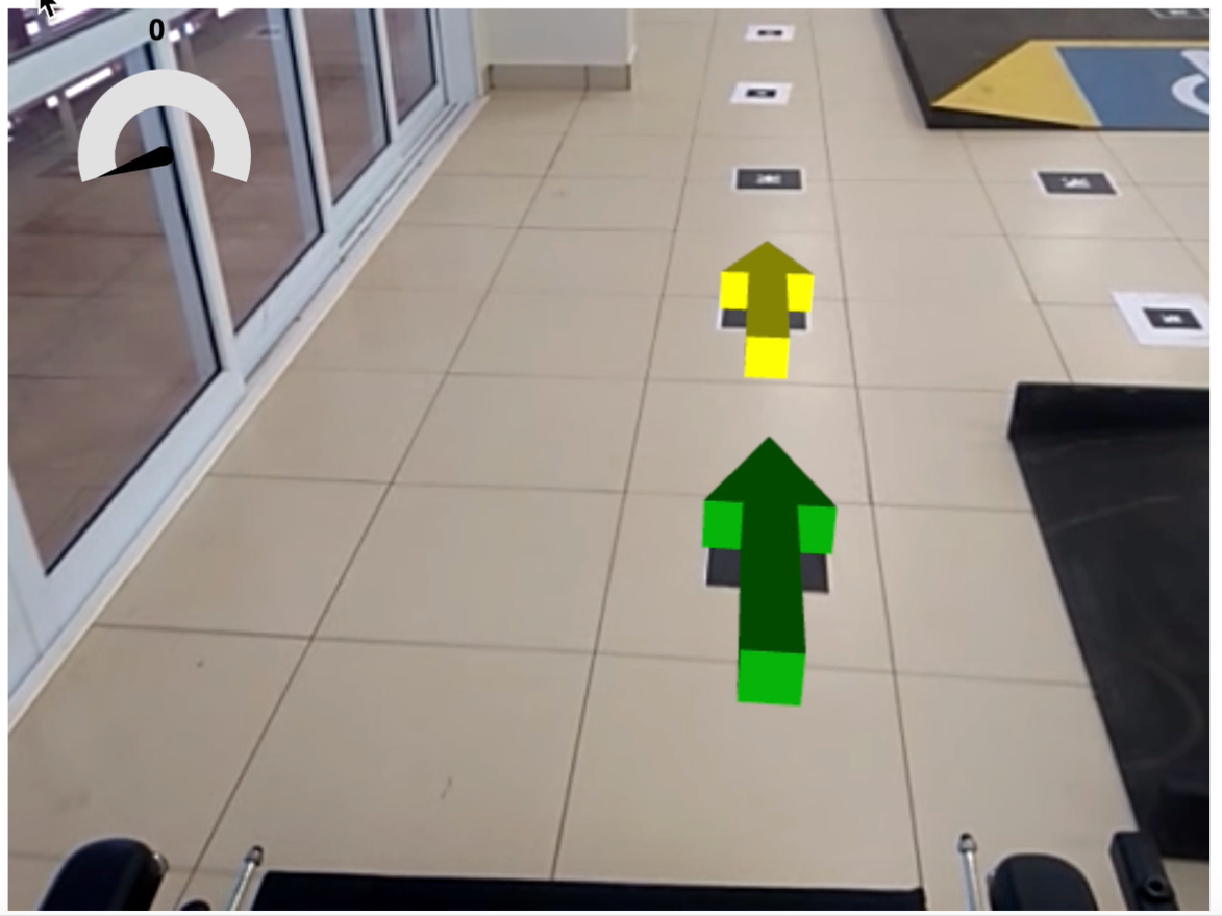
\includegraphics[width=1\linewidth]{img/cap6/endFirstAct}
\caption{End first activity} \label{fig:endFirstAct}
\end{minipage}
\begin{minipage}{0.495\linewidth}
\center
\captionsetup{justification=centering,margin=0cm,font=small}
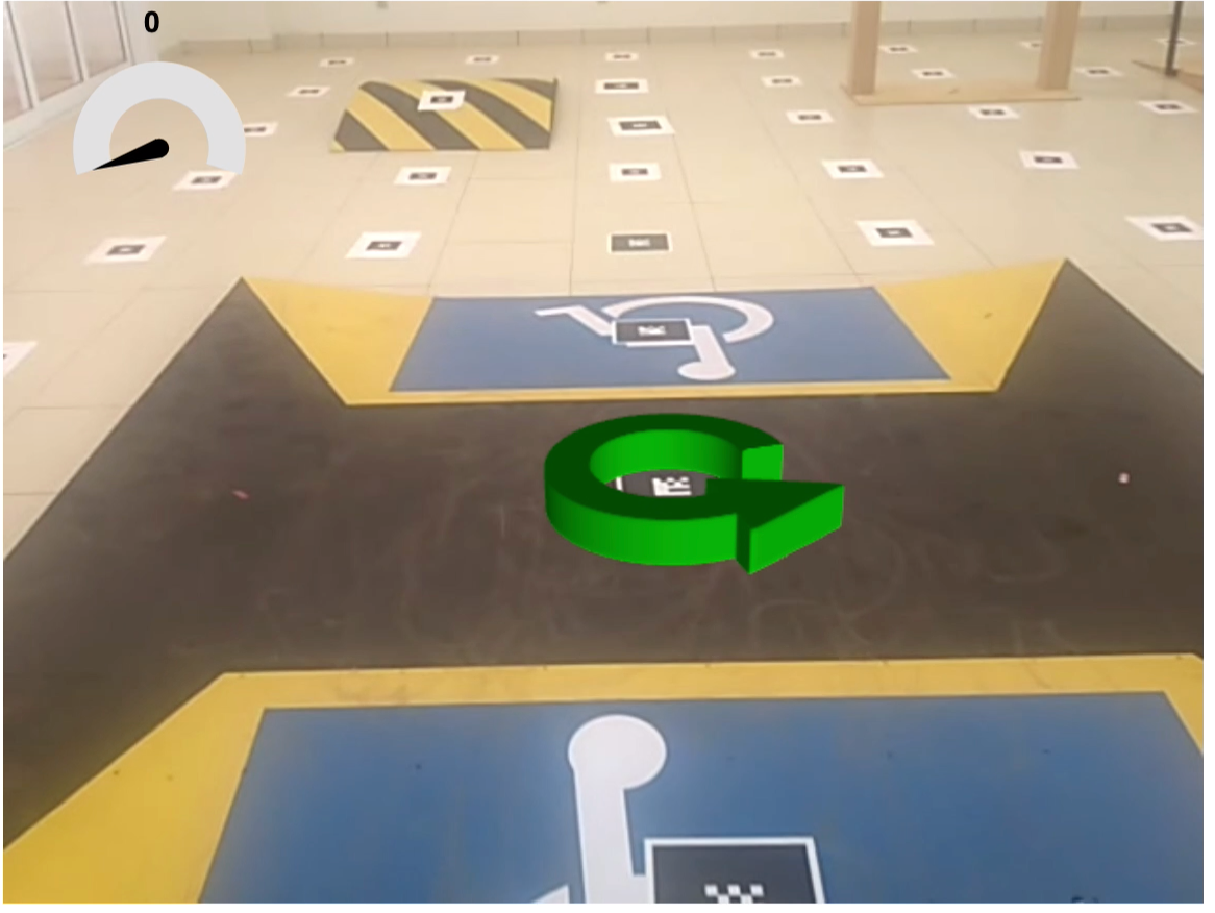
\includegraphics[width=1\linewidth]{img/cap6/spingWAct}
\caption{Spin the PW} \label{fig:spingWAct}
\end{minipage}
\end{figure}


During the execution of each training protocol, the therapist is able to monitor the participants’ performance in the proposed activities. Upon completion of the training process, the therapist must fill the adapted PMRT assessment form. Information such as number of commands and elapsed-time are retrieved from the database. The therapist must still fill in the number of collisions and comment on the participant’s performance, before assigning a score (4, 3, 2, or 1) to the activity, following the criteria established in Section \ref{sec:trainingEvaluation}. After each activity scores are applied, the final score of the protocol is calculated as described in Equation (\ref{eq:pmrtFinalScore}).   

\begin{equation}\label{eq:pmrtFinalScore}
Y = \sum_{i}^{n}\left (  \frac{x_{i}}{n*4}\right )* 100\%
\end{equation}

Where:
\begin{itemize}
\item Y: final score obtained;
\item n: tasks number defined for each training protocol;
\item i: present task index; and
\item $x_{i}$: present task value attributed;
\end{itemize}

The evaluation summary from the participants is presented by Table \ref{tb:ResultsPMRT} and as defined, a score greater the 95\% is needed to be considered approved \cite{massengale2005}. Nobody passed the experiments! Observing the criteria for grading and monitoring the participants training, it is understandable that this did not happen. Among them, some had severe collisions, or to complete the activity, they had to restart a maneuver several times. It reduces the task score value. But the objective was not to approve or not each participant but to demonstrate that the system also offers resources for user evaluation by the therapist. Also, the therapist can follow the evolution of the participant’s abilities through the comparative bar charts, shown in Figure \ref{fig:tGenerateChart}. Furthermore, he can define the design of future protocols that will prepare the user to drive a PW in their daily activities confidently.

\begin{figure}[!hbt]
\begin{center}
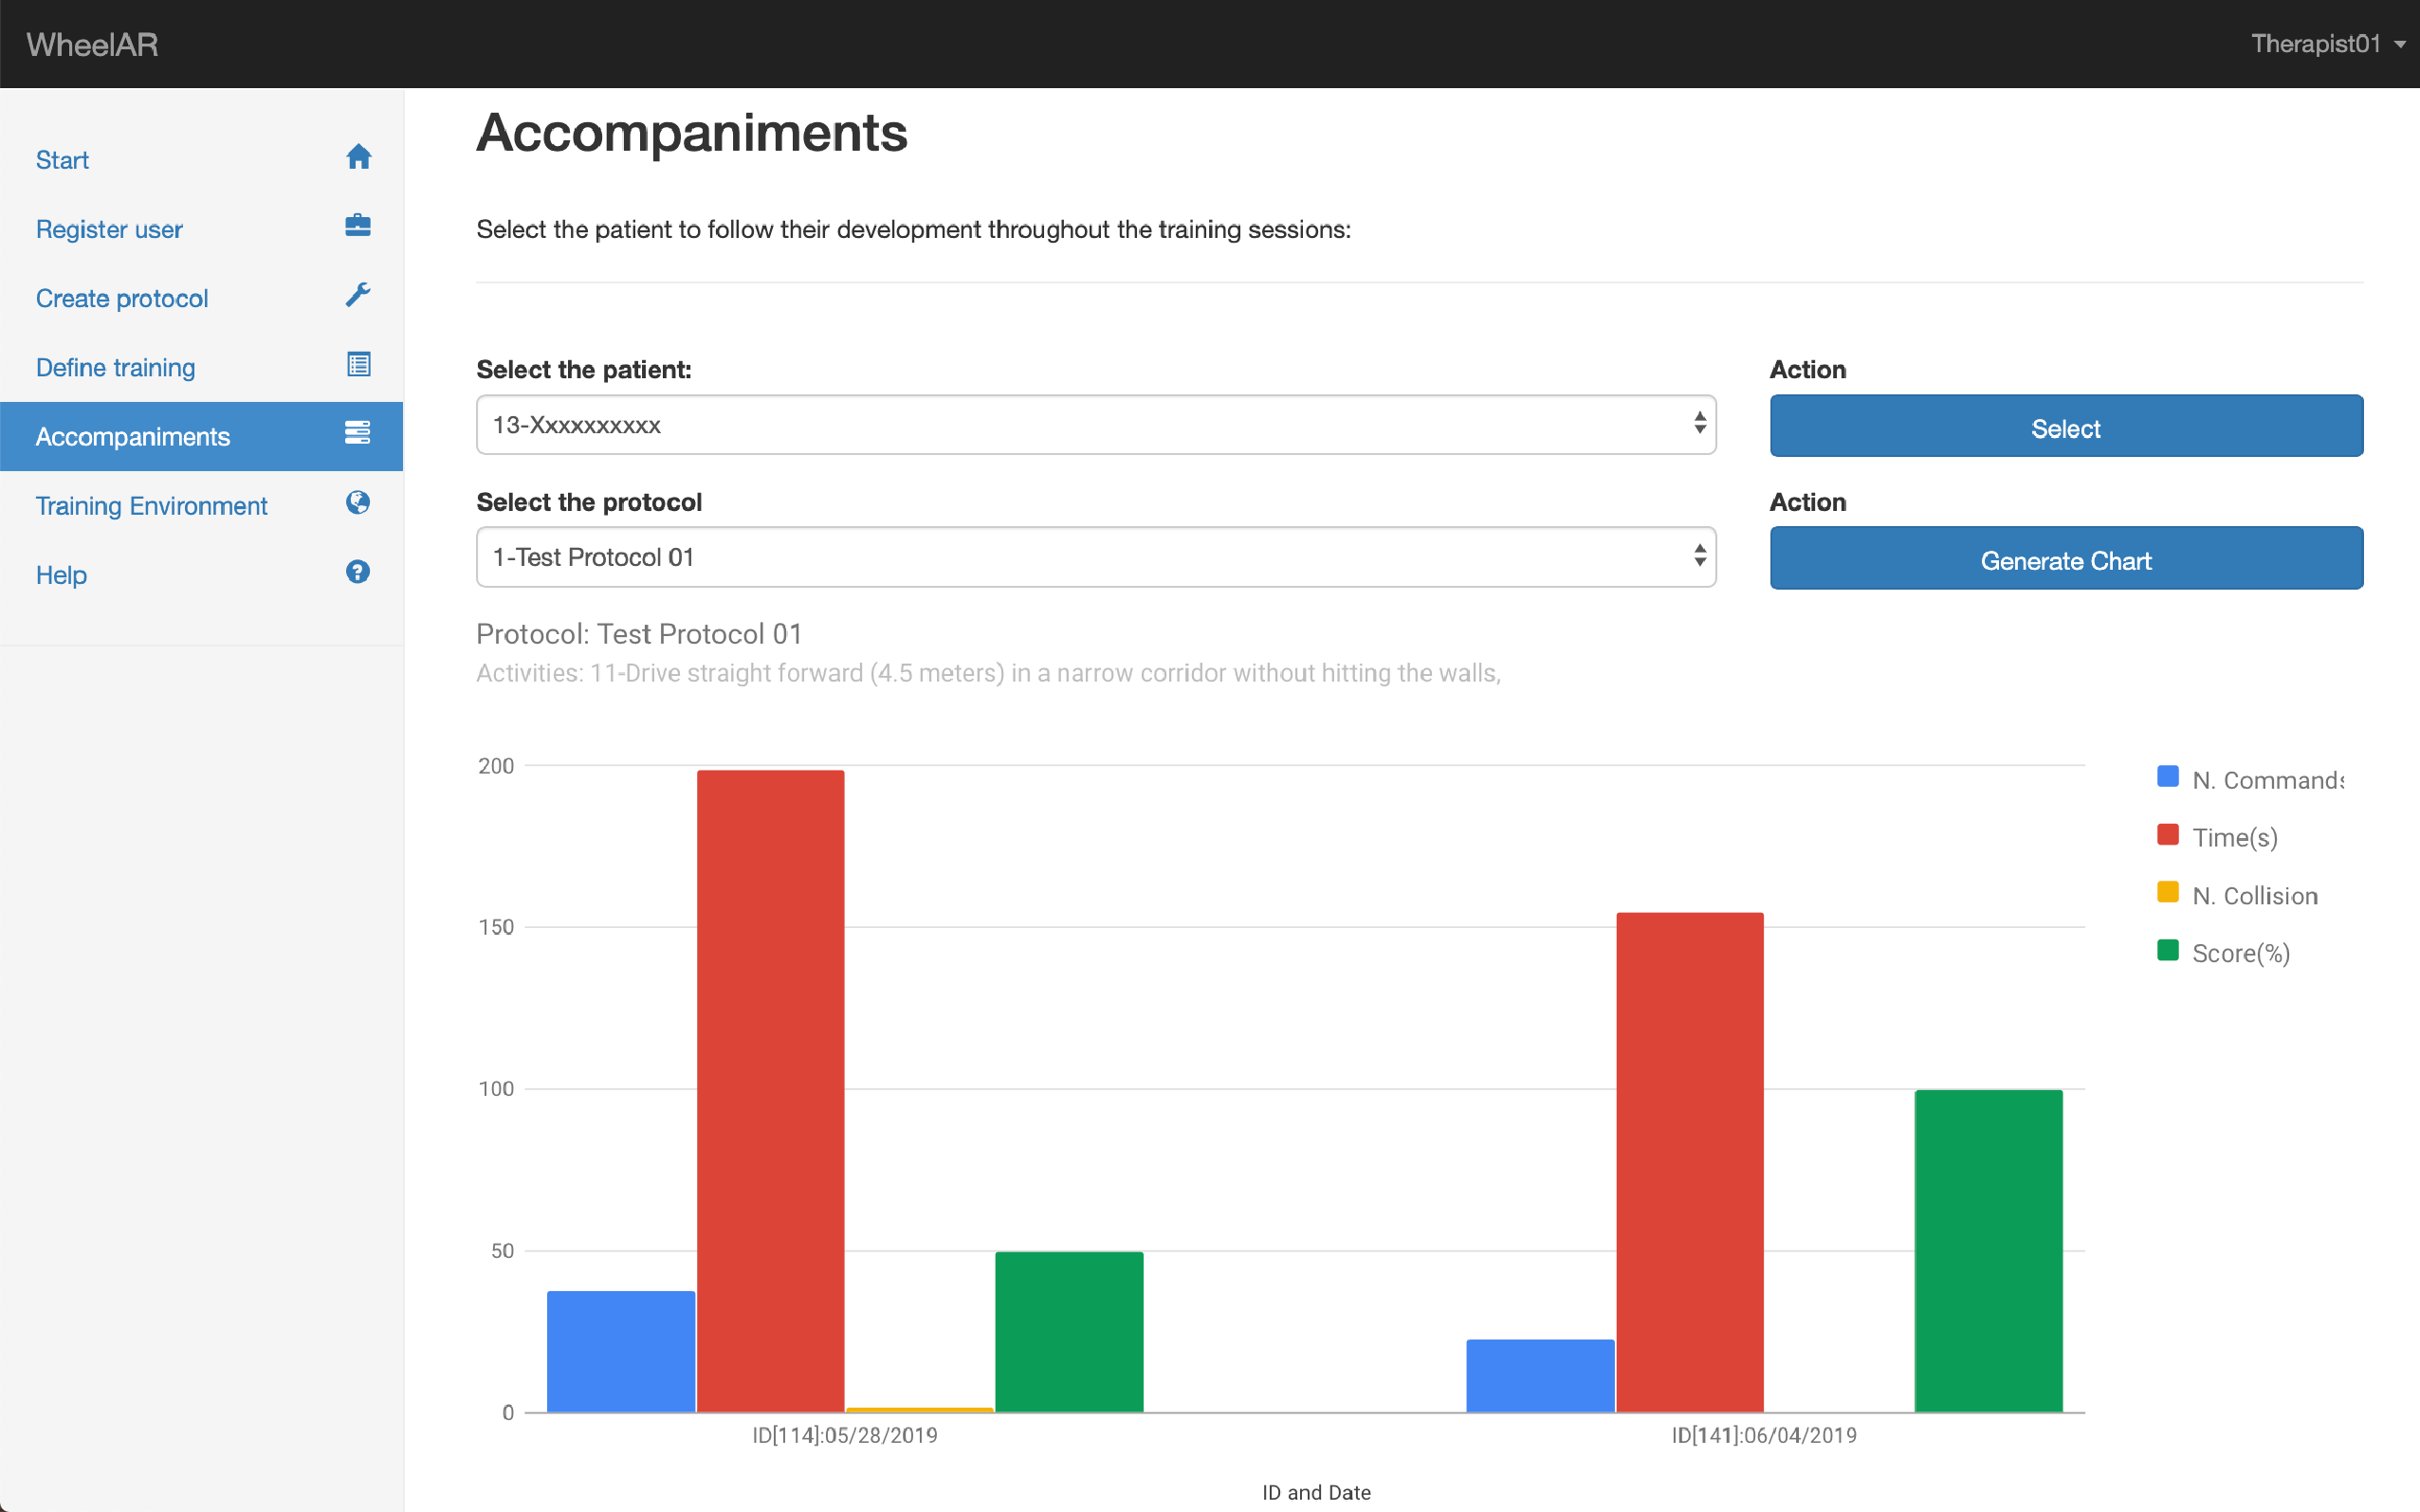
\includegraphics[width=1\linewidth]{img/cap6/tGenerateChart02}
\caption{User training protocol comparison} \label{fig:tGenerateChart}
\end{center}
\end{figure}


Biosignals can provide important information related to participant’s performance connected to the emotional state, which can prove useful in future training applications and on strategies for improving safety during PW use. 

The participant’s emotional state can constitute a barrier to good driving performance. Thus, it is important to understand, whenever these issues arise, whether the underlying cause is related to the participant’s motor skills or associated to their emotional state, looking to correctly address these issues. Additionally, in training protocols, it is desired that the user is not overwhelmed by the training difficulty level, which could be observed through his biosignals with appropriate methodology and detection algorithms. 

As can be seen from question 9 evaluation, none of the users felt tired after completing the proposed protocols. What allows us to observe another benefit made possible by the architecture, which is the adaptation of the PMRT, allowing the adjustment in the number of activities of the protocols.

This means that, in this specific case, there was no relevant difference on participants performance considering the three different protocols. However, this does not represent a final conclusion given that the sample was small and the protocol duration, considered as short - longer protocols, might present different results. The intention of this preliminary test is to show the system architecture capabilities. Having a different impact across individuals may emphasize the importance of having individualized or personalized protocols that could be based on therapist observations complemented by biosignal data.

\section{Final considerations}

First collaborations that the system brought to the participants are: increased well-being after each session, level of realism and immersion and still listening to the PW engines and collisions. All of this is due to the adaptation made in the PMRT merged with AR techniques, which allow the therapist to define a protocol that best suits the participant in real-time. Even though in this study, everyone used the same protocol. 

In addition, the analysis of biosignals was presented as a good assessment alternative because it allows realizing how deeper and challenging a protocol can be for a user, allowing for another assessment, which is not based on the therapist's visual analysis.

However, still talking about the system, a significant challenge encountered by all telerehabilitation systems was present: latency. It reduces the impression of real-time interaction with the increased environment. This is an Internet limitation, in general, some flaws, such as rendering objects, because the images have a reduced quality to maintain the connection.
However, the architecture already presents its potential for both therapists and users, but it still requires some improvements like fiducial AR marker recognition avoiding failure on virtual objects rendering, to exchange the current PW by another one with diagonal movements and promote studies about how to reduce latency effects on the video stream.

In the next section, general conclusions about the work and future improvement actions will be presented.

 